\graphicspath{{chapters/images/02/}}

\chapter{Second Week}

\section{Central Dogma}

\section{Measure biomolecules}
\textbf{Proteins}
\begin{itemize}
	\item Western blot
	\item ELISA
	\item Northern blot
	\item Enzyme assay
\end{itemize}\\


\textbf{RNA}
\begin{itemize}
	\item \textbf{DNA microarray}: it is an old technique
	\item RT-PCR
	\item \textbf{RNA sequencing} based on next generation sequencing  
\end{itemize}\\

\subsection{DNA microarrays}
points on a glass slide, technology invented in 1990s, they were developed after macroarrays.
The technology can be used to quantify miRNA, SNP excetera. It includes all the genes in the genome, including the splice variants and it is reliable for gene expression quantifications. It is easy to analyze, thanks to the bioinformatics resources that are now available.

\begin{figure}[h]
\caption{}
\centering
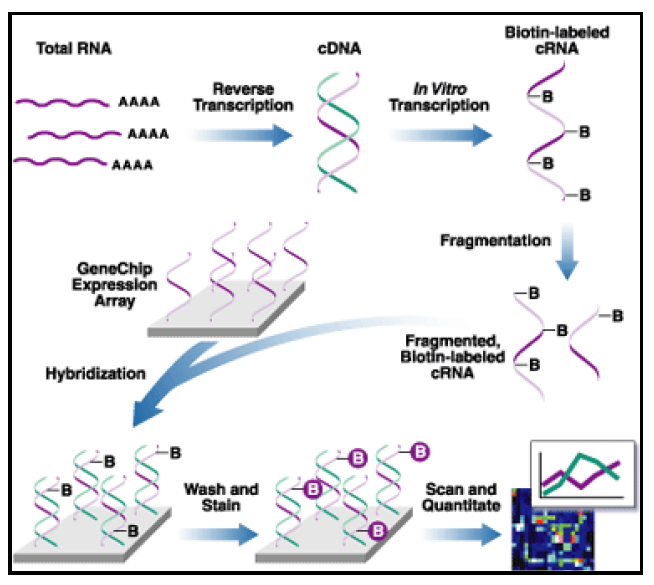
\includegraphics[width=0.6\textwidth]{microarrays}
\end{figure}

Affymatrix is a device that permits to do everything on a chip, it was developed for a series of species.\\
Competitor of Affimetrix is Illumina BeadChip, beads are ligated to oligonucleotides. The beads are inside wells. Illumina makes two colours cheaps (in terms of fluorescence). The possible source of errors are depicted in the image:
The first thing to do is to extract RNA from cells, which could be contaminated, then the extraction of RNA occurs, and a low extraction is possible. Degradation of RNA could also happen. During the reverse transcription, and fluorescent labelling, you have to ensure that the reverse transcription happen for each molecule, and each has to be labled. After, during hybridization has to occur equally for all the molecules, it could also happen cross-hybridization. Longer fragments can help in this. Scanning errors could also take place at the end.

\begin{figure}[h]
\caption{}
\centering
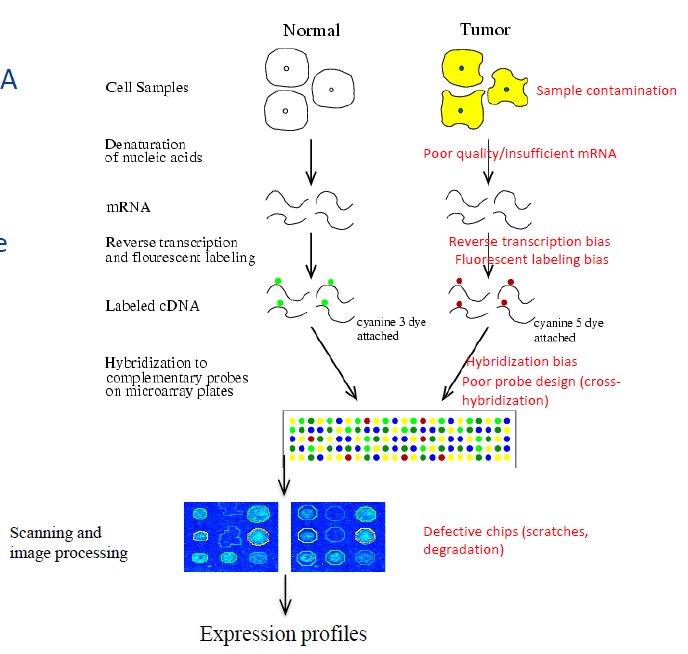
\includegraphics[width=0.6\textwidth]{ProblemsMicarrays}
\end{figure}

Other types of errors, can be due to non-specific fluorescence. Binding could also happen not specifically. Some methods exist to reduce the noise (error), for example: the Affy matrix, which uses two probes, one with Perfect Matches and a similar probe, but with a single different nucleotids (mismatch). If you subtract the two fluorescences, you should eliminate the noisy fluorescence (due to non-specific hybridizations).

At the end, it is obtained an \textbf{absolute quantification}.

identical Probe, and one which distinguish itself for a single mismatch. It is tried to remove the fluorescence which is not due to a specific hybridization. It is not very effective. 

Affymatrix give data for quality control check.   
what is RMA?  %TODO

spy probes hwich are not converted to a specific gene, If I'm analyzing human RNA, I can add mouse RNA.






Bioconductor?


\section{Normalization}
In addition to background correction, it can be done a normalization. It is made a boxplot, where each column represents a profile of the dataset, it represents the distribution of values in the dataset. Compare the distribution of values. It tries to realign the data, compute the avagare and subtract the avarage. 

Quantile normalization is more drastic. Other techniques are then possible.



\section{Other problems with transcriptomics}
\begin{itemize}
	\item certain ranges of values, if the expression of a gene is over this rang, it will be not possible to have a response.
	\item The gene might not be on the chip, 
	\item Can’t differentiate splice variants well. Some chips are designed to visualize only a part of a gene. Theere  are some specialized chips to do this, but normally this doesn't happen. YOu need to have the promoter of the gene. 
	\item The gene might be below detection limit
	\item Can’t differentiate RNA synthesis and degradation
	\item Can’t tell us about post translational events
	\item Bioinformatics can be difficult
\end{itemize}


Affymetrix GenexChip generates several type of files, such as •
DAT (image file), 
CEL (raw data file), 
CDF (chip definition file)
All platforms have different data formats. 

microarray standards like MIAME or MAGE-ML are STANDARDS ... %TODO




Bioconductor is a open source software project for the analysis and comprehension of genomic data. Provide  a wide range of powerful statistical andgraphical tools.



Microarrays can be found in repositories, like Array express, sited in UK, Gene Expression Omnibus, founded by NIH in USA, the japanese CIBEX, and other databases like NetAffx, Ensembl, TIGR, Stanford.... ArrayExpress and GEO have not overlapping pieces of data. Recount2 has small number of datasets, and most of them are also of GEO


\section{RNAseq}
it's an alternative way of measuring the level of expression of some genes, it uses next generation sequencing techniques. How this? it represents the toal technologies which permit to sequence an entire human genome in one week only, and of course with lower costs, if compared to the amount of money that was spent for the human genoe project. The speed and the cost are nowadays lowering.


At the beginning, long stratches of DNA sequenced, with this one instead the reads are really shorter (200 bases long around), but in much larger quantities. The idea is, if you want to quantify the messanger RNA of a cell, and sequence them, you have to split the nucleic acid: stretches thatare around 250 bases long.
To reassable, it is possible to take different samples, and for each one of them to perform a random fragmantation. Through computations, it is possible to reunify the reads. It is possible to quantify the messanger RNA molecules, to quantify the different splicing products. For the riassambly, a software is used 
 through these sequencings, it is possible to identify the reads.

RNA seq sequencing everything which is inside the cells. Requires computer with big rams and big storage to manage all the number of reads. With cloud computing it is possible to have thses problems solved. Recount provides datasets from GEOs. Raw counts are obtained from the first steps, preprocessing. It is produced a matrix, each row is a gene, each col a sample. Integer numbers. Different from the microarrays since here there are integers.

Several type of files,
FastQ is a text-file where each row is a sequence, produced by illumina sequencing machines. Different types of FastaQ files are produced. The BAM is a text-file with the read and next to it the coordinates with reference to the genome of sequencing. At the end the raw counts

now it is needed preprocessing, counts are treaky to handle. Confront samples, confront levels of expressions, inter-sample or intra-sample. Since counts, compare numbers? no, each run doesn't produce the same amount of reads. This means that it is not possible to compare the number presents. Normalize with respect total number of reads needed 

The bigger gene larger amounts of gene, normalize length reads and of genes. Some normalization processes are figured in the table below. RPM stands for Read per Million, normalize count per the total n of reads, RPKM normalizes gene length and mapped reads. Depending on hte order of normalization, one of the 2 results. TPM is slightly better.


Differential expression genes, t-test, which genes are affected by the changes. When the distance between averages is significant. To do a t-test, some other methods are to be applied. 


Description of the experiment gives us informations about the modality of analysis that should be considered to make the analysis, two groups, a control and a test group, minimally. 
Average experiments have replicates, to reduce the amount and the probability of errors, altough more expensive. 

\textbf{Guidelines}:
\begin{itemize}
	\item choose the data
	\item preliminary analysis
	\item normalization
	\item
\end{itemize} 

In order to make better decision, is to make interesting biological questions. 
%
%Bioconductor is an open source software project for the analysis %and comprehension %TODO




%\section{Alignment}
%It can be done by different types of aligners: 



%The
%most common application of RNA seq is to estimate gene transcript %expression. Aggregate
%raw counts of mapped reads
%(number of reads that successfully mapped to each
%gene/transcript  NOT for pseudoaligners






boxplot, column output of one microarray
normalization: to make values comparable, basically you compute median for each array and subtract the mean for that array. next divide all the values for the standard deviation, boxes nicely alligned and same space. This because assume the large majority of genes are not changing from a sample to another. Normalization tries to eliminate that error. Several file formats, the databases considered are GEO, attempt to standardize format of files, MIAME for example.

Recount2 takes dataset foundable in GEO, preprocess them

RNAseq is a different approach to quantify RNA. RNA molecules are cut with restriction enzymes, chop original RNA. Then, the library can be fed to the sequencing machine, which produces a very long file with the list of the fragments and their sequences. Re-assamble those fragments in order to obtain the original RNA. Re-assembly is easier thanks to a reference genome, sequence several version of the library: chopping in different ways, generation of different fragments. This augments the probability of overlapping. Computational intensive (Gb). Recount permits to have the raw counts, a matrix obtained after performing several action, each row a gene and column a sample, n of fragments associated to that gene. 
Idea of the level of expression of that gene. Difference with microarray matrix: integrals, relative count (on 10000000 reads, n fragments where seen to be related to that particular gene). The total number of reads have to be equal in each sample, otherwise normalization needed. The number of fragments augment if gene longer. Several methods to make comparisons between different samples. 
Depending on the normalization that I want, I need a specific package. 

microarray: limitation of the chip, design
RNA sequencing: no limitation, as everything is sequenced. extra computations.

microarray gives direct quantification of the mRNA. %da aggiungere alle altre caratteristiche


\section{Features of the selected database}
RNA sequencing data are those selected. mRNA is not able to tell us about the proteomics of a cell, as the degradative path is not weel studiable. 


dataset with two groups maybe, max 3 groups. A sufficient number of replicates have to be used to reduce errors. limited number of groups, large number of samples. Very large dataset, it can be taken a number of samples from the total dataset. At least 10 samples per group. Take or a dataset from Geo, or Array or structure.

Geo or ArrayExpress give preprocessed data. processed data in case of RNAseq are the raw counts. Other modifications are necessary. Why not giving the final results? Each step requires a decision about the algorithm to choose.


Assays are the samples


series file from GEO, open in excel. The number represents the probe ID, in fact, different probes can be used to find a gene. It is necessary to go from the probe to the gene. Different IDs represent different probes to find the gene. If you use microRNA datasets, you have to convert the microRNA to its genes. 

Recount3 contains tumor data,  

SRA is a repository for RNAseq data. It has only raw data, not preprocessed data. 

Series matrix file, check the data is in there. Geo could fail in case of absence of data. \textit{getGEO} can be used to find a file in the local directory.

If the RNAseq data are not shown in GEO, but there is an SRA reference, try to find the SRA ID in recount3